% !TeX document-id = {39d24ce0-844d-44a8-943b-2a9698211621}
% !TeX encoding = UTF-8
% !TeX spellcheck = en_US
% !TeX TXS-program:bibliography = biber -l zh__pinyin --output-safechars %
% !TeX TS-program = xelatex
%%% LuaLaTeX is required for `tikz-feynman`

\documentclass[a4paper,10pt]{article}

\newcommand{\hwNumber}{7}

% Templates: 82ccb576e4df24e5eac4194b76230be360b4f733

% to be `\input` in subfolders,
% ... therefore the path should be relative to subfolders.

\usepackage[UTF8
	,heading=false
	,scheme=plain % English Document
]{ctex}

\input{../.modules/basics/macros.tex}
\input{../.modules/preamble_base.tex}
\input{../.modules/preamble_notes.tex}

\newcommand{\legacyReference}{{
	\clearpage\par
	\quad\clearpage
	\renewcommand{\midquote}{\textbf{PAST WORK, AS TEMPLATE}}
	\newparagraph
}}

% Settings
\counterwithout{equation}{section}
\mathtoolsset{showonlyrefs=false}
%\DeclareTextFontCommand{\textbf}{\sffamily}
\renewcommand{\midquote}{\quad}

% Spacing
\geometry{footnotesep=2\baselineskip} % pre footnote split
\setlength{\parskip}{.5\baselineskip}
\renewcommand{\baselinestretch}{1.15}

%Title
	\posttitle{
		\hfill\Large\ccbyncsajp
		\par\end{flushleft}%
		\vspace*{-.7ex}\hrule%
	}
	\preauthor{\vspace{-1.5ex}%
		\flushleft\itshape%
	}
	\postauthor{\hfill}
	\predate{\noindent\ttfamily Compiled @ }
	\postdate{\vspace{.5ex}}

	\title{String Theory \textnumero\hwNumber}
	\author{\signature Bryan}
	\date{\today}

% List
	\setlist*{
		listparindent=\parindent
		,labelindent=\parindent
		,parsep=\parskip
		,itemsep=1.2\parskip
		,leftmargin=0pt
		,itemindent=*
	}
	\setlist*[enumerate,1]{
		align=left
		,label=\fbox{\textbf{\arabic*}}
		,itemsep=.5\baselineskip
		,itemindent=*
	}

\input{../.modules/basics/biblatex.tex}

%%% ID: sensitive, do NOT publish!
\InputIfFileExists{../id.tex}{}{}

\newcommand{\oppower}[2]{\mop{{#1}^{#2}}\!}
\newcommand{\sqsinh}{\oppower{\sinh}{2}}
\newcommand{\sqcosh}{\oppower{\cosh}{2}}

\newcommand{\Vir}{\mathbf{V}\mfrak{ir}}
\newcommand{\zbar}{\bar{z}}
%\usepackage{tikz-feynman,cancel}

% NS & R with spacing
\newcommand{\NS}{\ensuremath{\mspace{2mu}\mrm{NS}}}
\newcommand{\R}{\ensuremath{\mspace{2mu}\mrm{R}}}

% representations
\newcommand{\mbf}[1]{\mathbf{#1}}

%\addbibresource{strings6.bib}

\begin{document}
\maketitle
\pagestyle{headings}
\pagenumbering{arabic}
\thispagestyle{empty}

%{
%	\noindent\itshape%
%	本文约定:度规$\eta\sim\pqty{-,+,+,+}$, 指标$\mu,\nu,\dots = 0,1,2,3,\ i,j,\dots = 1,2,3$.
%}

\begin{enumerate}

\item \textbf{T-duality of Heterotic Strings}\footnote{
		I would like to thank Lucy Smith for help with this problem. 
	}
	
	We use $d \le 10$ to denote the number of noncompact dimensions; the remaining $m \ge d$ dimensions are compactified. For heterotic strings, the $I\ge 10$ dimensions of the left-moving sector are already compactified on a lattice $\Gamma_{16}$ or $\Gamma_8\times \Gamma_8$. Here we use the label $I$ to index the 16 internal dimensions. 
	
	\begin{enumerate}
	\item Generally, if we compactify an open string on the $x^m$ direction: $x^m \cong x^m + 2\pi R$ with constant backgrounds $A_m$, then its zero mode spectrum, \textit{with winding $w = 0$}, can be obtained from canonical quantization of the effective point particle action, with an additional gauge action term in the form of a Wilson line\footnote{
		Reference: \textit{Polchinski}, Chapter 8. 
	}:
	\begin{equation}
		-W_q
		= -iq \int \dd{x^m} A_m
		\sim -iq \int \dd{\tau} A_m \dot{X}^m
	\end{equation}
	By imposing that the canonical momentum to be periodic along $x^m$, we find that:
	\begin{equation}
		k_m = \frac{n_m}{R} - q A_m
	\label{eq:effective_momentum}
	\end{equation}
	
	To obtain the winding states, we have to reproduce the above action from the world-sheet description. For heterotic strings with $m < 10 \le I \le 26$, this can be achieved by adding the following term to the usual world-sheet action\footnote{
		Reference: \textit{Blumenhagen et al.}, Basic Concepts of String Theory. 
	}:
	\begin{equation}
		S_A \propto \int \dd[2]{\sigma}
			\epsilon^{ab} A^I_\mu
			\,\pdd{a} X^\mu
			\,\pdd{b} X_I
	\end{equation}
	With proper normalization to match the result in \eqref{eq:effective_momentum}. 
	
	Canonical quantization then produces\footnote{
		Reference: \textit{Polchinski}, Chapter 11. 
	}:
	\begin{gather}
		k_m
		= \frac{n_m}{R}
			\pm \frac{w_m R}{\alpha'}
			- q_I A^I_m
			- \frac{w_n R}{2} A^n_I A_m^I,
	\\
		k^I_L
		= \sqrt{\frac{2}{\alpha'}}\,
			\pqty{
				q^I + w^m R A^I_m
			},
	\end{gather}
	The \mquote{\pm} signs in $k_m$ correspond to the left and right-moving sector, respectively. Only the left-moving sector has an additional 16 dimensional internal torus, therefore $k^I$ is labeled with an $\mquote{L}$. 
	
	Note that the charge $q^I$ now takes value on the $\Gamma_{16}$ or $\Gamma_8\times \Gamma_8$ lattice, and:
	\begin{equation}
		l\circ l'
		= \frac{\alpha'}{2} \pqty{
				k^I_L\, k'_{L,I}
				+ k^m_L\, k'_{L,m}
				- k^m_R\, k'_{R,m}
			}
		= q^I q'_I
			+ 2nw
	\end{equation}
	We can then see that the new ``extended'' lattice indeed satisfies the even and self-dual conditions, which follows from the even and self-dual properties of $\Gamma_{16}$ or $\Gamma_8\times \Gamma_8$. 
	
	\item With $m = 9$ and $G_{dd} = 1$, we have:
	\begin{equation}
		W_q = \exp \pqty{-iq_I\theta^I},
	\quad
		A^I_9 = - \frac{\theta^I}{2\pi R}
	\end{equation}
	Note that $W_q$ captures the phase change of the paths that wind around $x^9$; the extra phase from a non-trivial Wilson line might affect the boundary condition of some states while leaving others intact, thus breaking the original gauge symmetry. Our discussions here closely follow \textit{Polchinski}, Chapter 11. 
	
	For the SO(32) theory with:
	\begin{equation}
		RA^I_9
		= \mop{diag} \pqty{
				(\tfrac{1}{2})^8,
				0^8
			}
	\end{equation}
	Adjoint states are labeled by a pair of indices valued in $1,\cdots,32$; those with one index from $1 \le A \le 16$ and one from $17 \le A \le 32$ are anti-periodic due to the additional phase $e^{i\pi} = -1$ from the Wilson line, so the gauge symmetry is reduced to $\mrm{SO}(16) \times \mrm{SO}(16)$. 
	
	Similarly, for the $E_8 \times E_8$ theory with:
	\begin{equation}
		R' A^I_9
		= \mop{diag} \pqty{
				1,0^7,
				1,0^7
			}
	\end{equation}
	Note that $\Gamma_8$, the root lattice of $E_8$, is basically the root lattice union an additional spinor weight lattice of SO(16). With the above Wilson line, the integer-charged states from the SO(16) root lattice in each $E_8$ remain periodic, while the half-integer charged states from the SO(16) spinor lattices become anti-periodic, due to the additional phase $e^{i\frac{1}{2}\cdot 2\pi} = -1$. Again the gauge symmetry is broken down to SO(16) × SO(16). 
	
	In summary, with the above Wilson line, the SO(32) and $E_8 \times E_8$ theory shares an unbroken gauge of SO(16) × SO(16). Consider the spectrum of the SO(16) × SO(16) \textit{neutral states}, i.e.\ those with internal momentum:
	\begin{equation}
		k^I_L
		= \sqrt{\frac{2}{\alpha'}}\,
			\pqty{
				q^I + w R A^I_9
			}
		= 0
	\end{equation}
	For the $\mrm{SO}(32)$ theory, since $q^I \in \Gamma_{16}$
%	or $\Gamma_8\times \Gamma_8$ 
%	and adjoint states in  are integer-charged 
	while $
		RA^I_9
		= \mop{diag} \pqty{
				(\tfrac{1}{2})^8,
				0^8
			}
	$, we must have $w = 2m$ for this to hold. The same goes for the $E_8 \times E_8$ theory;
	therefore, we have:
	\begin{gather}
		k_{L,R} = \frac{\tilde{n}}{R}
			\pm \frac{2mR}{\alpha'},
	\quad
		k'_{L,R} = \frac{\tilde{n}'}{R'}
			\pm \frac{2m'R'}{\alpha'},
	\\
		\tilde{n} = n + 2m,\quad
		\tilde{n}' = n' + 2m'
	\end{gather}
	
	\item If the two theories are related by T-duality, then we should expect:
	\begin{equation}
		(k_L, k_R) \longleftrightarrow (k'_L, −k'_R),
	\end{equation}
	Under suitable mapping of parameters. Indeed, it is straightforward to verify that $
		(\tilde{n},m)\leftrightarrow (m',\tilde{n}')
	$ realizes this, along with $
		RR' = \alpha'/2
	$. The above arguments can then be generalized to higher levels, by acting on fermionized left-moving fields $\lambda^A$ and carefully organizing representations. We see that the two heterotic string theories are equivalent under T-duality.
	\end{enumerate}

\item \textbf{String Junction}\footnote{
		Reference: \arxiv{0812.4408}. 
	}
%	\begin{figure}[!ht]
%	\centering
%	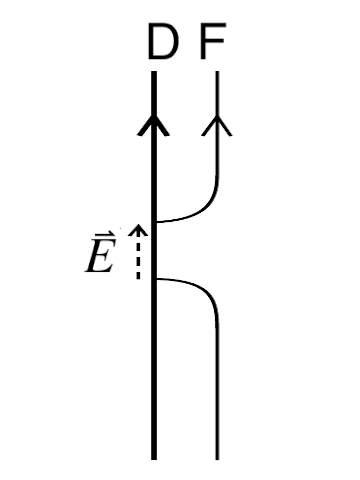
\includegraphics[width=.2\linewidth]{FD_bound.png}
%	\caption{String Junction}
%	\label{fig:string_junction}
%	\end{figure}
	
	\nopagebreak
	For a string junction to be mechanically stable, the tension force exerted on the junction must cancel each other; this is a Newtonian mechanics problem, but with $(p,q)$-string tension given by the BPS bound:
	\begin{equation}
		\tau_{(p,q)}
		= \frac{\sqrt{p^2 + q^2/g^2}}{2\pi\alpha'}
	\end{equation}
	Stability of the system implies that the BPS bound should be saturated. 
	
	From Newtonian mechanics, we know that three forces cannot cancel each other unless they are co-planar. Therefore, a 3-string junction must be co-planar in order to be stable. Suppose they lie in the $(X^1,X^2)$ plane, then the tension exerted on the junction can expressed as:
	\begin{equation}
		\vec{T}_i = \tau_{(p_i,q_i)}\,\pqty{
				\cos\theta_i,
				\sin\theta_i
			},
	\quad i = 1,2,3,
	\end{equation}
	$\sum_i \vec{T}_i = 0$ gives two equations, and we have two independent unknowns (the angle between two pairs of strings); therefore if a solution exists, it should be unique up to rotations and reflections. 
	
	In fact, a solution can be found by simple observations:
	\begin{equation}
		\cos\theta_i
		= \frac{p_i}{\sqrt{p^2 + q^2/g^2}},
	\quad
		\sin\theta_i
		= \frac{q_i/g}{\sqrt{p^2 + q^2/g^2}},
	\end{equation}
	It satisfies $\sum_i \vec{T}_i = 0$ since that total $(p,q)$ vanishes at each junction. 
	
	To find the remaining supersymmetries of this system, we start from the original supersymmetries of a $(p,q)$ string (which saturates the BPS bound) extended along the $\hat{X} = (\cos\theta,\sin\theta)$ direction:
	\begin{gather}
		\frac{1}{2L\tau_{(p,q)}} \Bqty{
			\bqty{\mqty{
				Q_\alpha \\
				\tilde{Q}_\alpha
			}},
			\bqty{
				Q^\dagger_\beta
				\ \tilde{Q}^\dagger_\beta}
		}
		= \delta_{\alpha\beta}
				\bmqty{
					1 & 0 \\
					0 & 1 \\
				}
			+ (\Gamma^0 \Gamma^\theta)_{\alpha\beta}
				\bmqty{
					\cos\theta & \sin\theta \\
					\sin\theta & -\cos\theta \\
				},
	\\
		\Gamma^\theta
		= \hat{X}\cdot \vec{\Gamma}
		= \Gamma^1\cos\theta + \Gamma^2\sin\theta
	\end{gather}
	We see that the algebra depends on $\theta$, i.e.\ it is different for strings in different directions. However, if we can find a (maximal) subalgebra that is independent of $\theta$, then we would have found the remaining supersymmetries of the full system\footnote{
		The $\tau_{(p,q)}$ factor can be absorbed by rescaling generators, hence does not matter in our discussions. 
	}. 
	
	We begin with diagonalizing the matrix on the RHS with:
	\begin{gather}
		U(\tfrac{\theta}{2}) = \bmqty{
				\cos\frac{\theta}{2} &
				-\sin\frac{\theta}{2} \\
				\sin\frac{\theta}{2} &
				\cos\frac{\theta}{2} \\
			},
	\\[1ex]
		\frac{1}{2L\tau_{(p,q)}} \Bqty{
			U^{\mrm{T}}
			\bqty{\mqty{
				Q_\alpha \\
				\tilde{Q}_\alpha
			}},
			\bqty{
				Q^\dagger_\beta
				\ \tilde{Q}^\dagger_\beta
			}
			U
		}
		= \bmqty{
			(\idty + \Gamma^0\Gamma^\theta)_{\alpha\beta} &
			0 \\
			0 &
			(\idty - \Gamma^0\Gamma^\theta)_{\alpha\beta} \\
		},
	\end{gather}
	Note that $
		(\idty + \Gamma^0\Gamma^\theta)
		(\idty - \Gamma^0\Gamma^\theta)
		= 0
	$ and $
		(\idty + \Gamma^0\Gamma^\theta)
		+ (\idty - \Gamma^0\Gamma^\theta)
		= 2\idty
	$, i.e.\ they are orthogonal to each other; acting $
		(\idty \pm \Gamma^0\Gamma^\theta)
	$ on both sides, we find the following combinations, which gives the 16 SUSYs of a $(p,q)$ string:
	\begin{equation}
		(\idty - \Gamma^0\Gamma^\theta)
		\pqty{
			\cos\tfrac{\theta}{2}\, Q
			+ \sin\tfrac{\theta}{2}\, \tilde{Q}
		}_\alpha
		= 0 =
		(\idty + \Gamma^0\Gamma^\theta)
		\pqty{
			- \sin\tfrac{\theta}{2}\, Q
			+ \cos\tfrac{\theta}{2}\, \tilde{Q}
		}_\beta
	\label{eq:pq_string_susy}
	\end{equation}
	
\pagebreak[4]
	
	For further simplification, we can isolate the $\theta$ dependence in $\Gamma^\theta$ by working in a specific representation of the Clifford algebra, e.g.\ the Dirac representation given by \textit{Polchinski}. Then $\alpha$ is given by 10\,D spinor components: $
		\alpha = (s_0,s_1,s_2,s_3,s_4),\ %
		s_i = \pm
	$, with additional chirality constraints from both $Q$ and $\tilde{Q}$: $
		\prod_i s_i = +
	$. In the end, we have 16 independent components as expected. 
	
	Details of the expansion are given in \arxiv{0812.4408}. When the dust settles, we find that the 16 SUSYs in \eqref{eq:pq_string_susy} is given by:
	\begin{subequations}
	\begin{gather}
		\sin\tfrac{\theta}{2}\,
		\pqty{
			\cos\tfrac{\theta}{2}\, Q
			+ \sin\tfrac{\theta}{2}\, \tilde{Q}
		}_{(++s)}
		+ \cos\tfrac{\theta}{2}\,
		\pqty{
			\cos\tfrac{\theta}{2}\, Q
			+ \sin\tfrac{\theta}{2}\, \tilde{Q}
		}_{(--s)},
	\\
		\sin\tfrac{\theta}{2}\,
		\pqty{
			\cos\tfrac{\theta}{2}\, Q
			+ \sin\tfrac{\theta}{2}\, \tilde{Q}
		}_{(+-s)}
		- \cos\tfrac{\theta}{2}\,
		\pqty{
			\cos\tfrac{\theta}{2}\, Q
			+ \sin\tfrac{\theta}{2}\, \tilde{Q}
		}_{(-+s)},
	\\
		\cos\tfrac{\theta}{2}\,
		\pqty{
			- \sin\tfrac{\theta}{2}\, Q
			+ \cos\tfrac{\theta}{2}\, \tilde{Q}
		}_{(++s)}
		- \sin\tfrac{\theta}{2}\,
		\pqty{
			- \sin\tfrac{\theta}{2}\, Q
			+ \cos\tfrac{\theta}{2}\, \tilde{Q}
		}_{(--s)},
	\\
		\cos\tfrac{\theta}{2}\,
		\pqty{
			- \sin\tfrac{\theta}{2}\, Q
			+ \cos\tfrac{\theta}{2}\, \tilde{Q}
		}_{(+-s)}
		+ \sin\tfrac{\theta}{2}\,
		\pqty{
			- \sin\tfrac{\theta}{2}\, Q
			+ \cos\tfrac{\theta}{2}\, \tilde{Q}
		}_{(-+s)},
	\end{gather}
	\end{subequations}
	\vspace{-.8\baselineskip}
	\begin{equation}
		s = (s_2 s_3 s_4),\quad
		\prod_i s_i = +
	\end{equation}
	
	By trial and error, we can find the 8 linear combinations that are independent of $\theta$; they are:
	\begin{gather}
		(a) + (c)
		\quad\Longrightarrow\quad
		\tilde{Q}_{(++s)} + Q_{(--s)},
	\\
		(b) + (d)
		\quad\Longrightarrow\quad
		\tilde{Q}_{(+-s)} - Q_{(-+s)},
	\end{gather}
	Therefore, the string junction is $\frac{8}{32} = \frac{1}{4}$ BPS. 

\item \textbf{Two and Three-Point Functions in AdS/CFT}
\def\adsFive/{$\mrm{AdS}_5$}
	
	Consider a scalar field $\phi(x,z)$ in Poincar\'e \adsFive/ (with radius $R = 1$) satisfying:
	\begin{equation}
		\pqty{\laplacian - m^2}\,
			\phi(x,z) = 0,
	\quad
		\phi(x,z) \to
		\left\lbrace\vbox to 12.5pt {}\right.
		\begin{aligned}
			& z^\delta \phi_0(x)\,,
				&& z\to 0, \\[-.35ex]
			& \mrm{regular},
				&& z\to\infty,
		\end{aligned}
	\quad
		\delta = 2 - \sqrt{m^2 + 4}
	\end{equation}
	It can be constructed via the boundary-to-bulk propagator $K_\Delta$:
	\begin{gather}
		\phi(x,z)
		= \int \dd[4]{x'}
			K_\Delta(x,z;x')\,
			\phi(x'),
	\\
		K_\Delta(x,z;x')
		= \frac{(\Delta - 1)(\Delta - 2)}{\pi^2}
			\pqty{\frac{z}{
				z^2 + \norm{x - x'}^2
			}}^{\!\!\Delta},
	\quad
		\Delta = 2 + \sqrt{m^2 + 4}
	\end{gather}
	
	\begin{enumerate}
	\item To verify this, we first check that the boundary conditions are indeed satisfied by $K_\Delta$; note that $\Delta \ge 2 > 0$, and we have:
	\begin{equation}
		z\to 0,\quad l \ne 0,
	\quad
		\pqty{\frac{z}{
			z^2 + l^2
		}}^{\!\!\Delta} \to 0,
	\end{equation}
	i.e.\ the only contribution comes from the $l\to 0$ case, where we have:
	\begin{equation}
	\begin{aligned}
		l = \norm{x - x'} \to 0,
	\quad
		\int \dd[4]{x'}
			K_\Delta(x,z;x')
		&= \frac{(\Delta - 1)(\Delta - 2)}{\pi^2}
			\int_0^\infty 2\pi^2 l^3 \dd{l}
				\pqty{\frac{z}{
					z^2 + l^2
				}}^{\!\!\Delta} \\
		&= \frac{(\Delta - 1)(\Delta - 2)}{\pi^2}\cdot
			\frac{2\pi^2}{2\,(\Delta - 1)(\Delta - 2)}\,
			z^{4 - \Delta} \\
		&= z^\delta
	\end{aligned}
	\end{equation}
	Therefore, we have:
	\begin{equation}
		z \to 0,
	\quad
		K_\Delta(x,z;x')
		\to z^\delta \delta^4(x - x'),
	\quad
		\phi(x,z)
		\to z^\delta \phi_0(x),
	\end{equation}
	The other boundary condition is convenient to check; we have:
	\begin{equation}
		z \to \infty,
	\quad
		K_\Delta(x,z;x')
		\propsim z^{-\Delta} \to 0,
	\quad
		\phi(x,z)
		\,\ \text{regular.}
	\end{equation}
	
	Now we need only check that $K_\Delta$ satisfies the equation of motion; in Poincar\'e \adsFive/ we have:
	\begin{equation}
		\laplacian
		= z^2 \pqty{
				\pdd{z}^2
				- \frac{3}{z}\, \pdd{z}
				+ \pdd{x}^2
			}
	\end{equation}
	With the help of Mathematica\textsuperscript{TM}, it is straightforward to check that $
		\pqty{\laplacian - m^2}\,
			\pqty\big{\frac{z}{
				z^2 + l^2
			}}^{\Delta}
		= 0
	$, therefore $
		\pqty{\laplacian - m^2}\,
			\phi(x,z) = 0
	$. 
	
	\newparagraph
	The AdS/CFT dictionary is given by:
	\begin{equation}
		\ave*{
			e^{
				\int\dd[4]{x}\,
					C_O\, \phi_0(x)\, O(x)
			}
		}_{\mrm{CFT}}
		= e^{-S[\phi_0]}
	\end{equation}
	Where $S[\phi_0]$ the bulk effective action evaluated on the solution to the equation of motion:
%	We have taken the classical limit in the RHS, since the AdS/CFT correspondence is a strong/weak duality; for a strongly coupled CFT the bulk theory is weakly coupled, 
	\begin{equation}
		S[\phi_0]
		= \int \dd[4]{x} \dd{z}
			\sqrt{-G}\,\Bqty{
				\frac{1}{2}\,\pqty{\pdd{\mu}\phi}^2
				+ \frac{1}{2}\,m^2 \phi^2
				+ \frac{1}{3}\,g \phi^3
				+ \cdots
			}
	\end{equation}
	
	\item The CFT 2-point function $
		\ave{O(x)\,O(y)}
	$ can be computed with the above dictionary, using the usual effective formalism, but with the bulk action instead of the boundary action:
	\begin{equation}
		\ave{O(x)\,O(y)}
		= \frac{1}{C_O^2}
			\eval{
				\frac{\var[2]}{
					\var{\phi_0(x)} \var{\phi_0(y)}
				}\, e^{-S[\phi_0]}
			}_{\phi_0=0}\!\!
	\end{equation}
	For 2-point function, we only need terms $\sim\order{\phi^2}$; note that:
	\begin{equation}
		\fdv{\phi(x,z)}{\phi_0(x')}
		= K_\Delta(x,z;x'),
	\end{equation}
	\vspace{-.5\baselineskip}
	\begin{equation}
	\begin{aligned}
		\var{S}[\phi_0]
		&\sim \int \dd[4]{x} \dd{z} \sqrt{-G}\,
				\pqty{-\laplacian + m^2}\,\phi \var{\phi}
			+ \int_{z\to 0} \dd[4]{x} \sqrt{-G}\,
				\pd^{z} \phi \var{\phi} \\
		&= 0 - \int_{z\to 0} \dd[4]{x}
				z^{-5} z^2
				\pdd{z} \phi \var{\phi}
		= -\int_{z\to 0} \dd[4]{x}
				z^{-3}
				\pdd{z} \phi \var{\phi},
	\end{aligned}
	\end{equation}
	\begin{equation}
	\begin{aligned}
		\therefore\quad
		\ave{O(x)\,O(y)}
		&= +\frac{1}{C_O^2}
			\eval{
				\frac{\var}{
					\var{\phi_0(x)}
				}\, e^{-S[\phi_0]}
				\int_{z\to 0} \dd[4]{x'} z^{-3}
					\pdd{z} \phi(x',z)\,
					K_\Delta(x',z;y)\,
			}_{\phi_0=0}\!\! \\
		&= \frac{1}{C_O^2}
				\int_{z\to 0} \dd[4]{x'} z^{-3}
					\pdd{z} K_\Delta(x',z;x)\,
					K_\Delta(x',z;y) \\
		&= \frac{1}{C_O^2}
				\int_{z\to 0} \dd[4]{x'} z^{-3}
					\pdd{z} K_\Delta(x',z;x)\,
					z^\delta \delta^4(x' - y) \\
		&= \frac{z^{\delta - 3}}{C_O^2}\,
			\pdd{z} K_\Delta(x,z;y) \\
		&\sim \frac{z^{\delta-3}}{C_O^2}\,
			\frac{(\Delta - 1)(\Delta - 2)}{\pi^2}
			\frac{
				\Delta z^{\Delta-1}
			}{\norm{x - y}^{2\Delta}} \\
		&= \frac{1}{C_O^2}\,
			\frac{\Delta(\Delta - 1)(\Delta - 2)}{\pi^2}
			\frac{1}{\norm{x - y}^{2\Delta}} \\
	\end{aligned}
	\end{equation}
	
	Therefore, if we want $
		\ave{O(x)\,O(y)}
		= \frac{1}{\norm{x - y}^{2\Delta}}
	$, then we have\footnote{
		Reference: \arxiv{hep-th/9804058}. Again I would like to thank Lucy Smith for helpful hints. 
	}:
	\begin{equation}
		C_O
		= \frac{1}{\pi} \sqrt{
				\Delta(\Delta - 1)(\Delta - 2)
			}
	\end{equation}
	Here $z\to 0$ is a cutoff parameter. 
	
	\item Similarly, we can use the dictionary to compute 3-point functions; we have\footnote{
		Reference: \arxiv{hep-th/9905111}, and \arxiv{hep-th/9804058}. 
	}:
	\begin{equation}
		\ave{O(x_1)\,O(x_2)\,O(x_3)}
		= \frac{1}{C_O^3}\,
			\pqty{-\frac{g}{3}}
			\int \dd[4]{x} \dd{z} \sqrt{-G}\,
				K_\Delta(x,z;x_1)\,
				K_\Delta(x,z;x_2)\,
				K_\Delta(x,z;x_3)
	\end{equation}
	This is a difficult integral; as is suggested by \arxiv{hep-th/9804058}, we can use an important symmetry of AdS/CFT --- the inversion $
		\vec{x}\mapsto \frac{\vec{x}}{x^2}
	$, to complete the integration. 
	
	By conformal symmetry, we know that the 3-point function is of the form:
	\begin{equation}
		\ave{O(x_1)\,O(x_2)\,O(x_3)}
		= A(x_1,x_2,x_3)
		= \frac{C_{OOO}}{
				\abs{x_{12}}^\Delta
				\abs{x_{23}}^\Delta
				\abs{x_{31}}^\Delta
			},\quad x_{ij} = x_i - x_j
	\end{equation}
	First set $x_3 = 0$, then perform inversion on all other points:
	\begin{gather}
		x_i = \frac{x'_i}{x'^2_i}, \quad
		(x,z) = \frac{(x',z')}{\,r'^2},
	\quad
		r^2 = x^2 + z^2,\quad
		r^2 r'^2 = 1 = x_i^2 x_i'^2,
	\\
		\frac{\dd[4]{x} \dd{z}}{z^5}
		= \frac{\dd[4]{x'} \dd{z'}}{z'^5},
	\\
	\begin{aligned}
		\frac{z}{z^2 + \norm{x - x_i}^2}
		&= \frac{z}{r^2 + x_i^2 - 2x\cdot x_i}
		= \frac{z'/r'^2}{
				1/r'^2 + 1/x'^2_i
				- 2x'\cdot x'_i/\pqty{r'^2 x'^2_i}
			} \\
		&= \frac{z'}{r'^2 + x'^2_i - 2x'\cdot x'_i}
			\,x'^2_i
		= \frac{z'}{z'^2 + \norm{x' - x'_i}^2}
			\,x'^2_i,
	\end{aligned}
	\\[1ex]
		K_\Delta(x,z;x_i)
		= K_\Delta(x',z';x'_i)\,\abs{x'_i}^{2\Delta}
		= \frac{1}{\abs{x_i}^{2\Delta}}\,
			K_\Delta(x',z';x'_i),
	\end{gather}
	With these in mind, we find that:
	\begin{equation}
		A(x_1,x_2,0)
		= -\frac{g}{3C_O^3}\,
			\frac{1}{\abs{x_1}^{2\Delta}}
			\frac{1}{\abs{x_2}^{2\Delta}}
			\frac{(\Delta - 1)(\Delta - 2)}{\pi^2}
		\int \frac{\dd[4]{x'} \dd{z'}}{z'^5}
			K_\Delta(x',z';x'_1)\,
			K_\Delta(x',z';x'_2)\,
			z'^\Delta
	\end{equation}
	The integral can then be completed using Feynman parameters; in the end we obtain:
	\begin{gather}
		A(x_1,x_2,0)
		\propto
			\frac{1}{\abs{x_1}^{2\Delta}}
			\frac{1}{\abs{x_2}^{2\Delta}}
			\frac{1}{\abs{x'_1 - x'_2}^{2\Delta}}
		= \frac{1}{
				\abs{x_1}^{\Delta}
				\abs{x_2}^{\Delta}
				\abs{x_1 - x_2}^{\Delta}
			},
	\\[1ex]
		C_{OOO}
		= -\frac{g}{3C_O^3}\,
			\frac{1}{2\pi^4}
			\pqty{
				\frac{\Gamma(\tfrac{\Delta}{2})}{
					\Gamma(\Delta - 2)
				}
			}^{\!\!3}
			\Gamma\pqty{
				\frac{3\Delta - 4}{2}
			}
	\end{gather}
	
	\end{enumerate}

\end{enumerate}

\printbibliography[%
%	title = {参考文献} %
	,heading = bibintoc
]
\end{document}
